\documentclass{beamer}
\usepackage{amsmath}
\usepackage{graphicx}
\usepackage{subfigure}

%\usepackage{caption}
%\usepackage{subcaption}

% Copyright 2004 by Till Tantau <tantau@users.sourceforge.net>.
%
% In principle, this file can be redistributed and/or modified under
% the terms of the GNU Public License, version 2.
%
% However, this file is supposed to be a template to be modified
% for your own needs. For this reason, if you use this file as a
% template and not specifically distribute it as part of a another
% package/program, I grant the extra permission to freely copy and
% modify this file as you see fit and even to delete this copyright
% notice. 


\mode<presentation>
{
  \usetheme{default}
  % or ...

  \setbeamercovered{transparent}
  % or whatever (possibly just delete it)
}


\usepackage[english]{babel}
% or whatever

\usepackage[utf8]{inputenc}
% or whatever

\usepackage{xcolor}
\usepackage[percent]{overpic}

\usefonttheme{serif}
\usecolortheme{seahorse}

\usepackage[T1]{fontenc}


\begin{document}
\begin{frame}{Active Feedback Resonator}
{\tiny Ouroboros}
%\begin{columns}
%\column{0.5\textwidth}
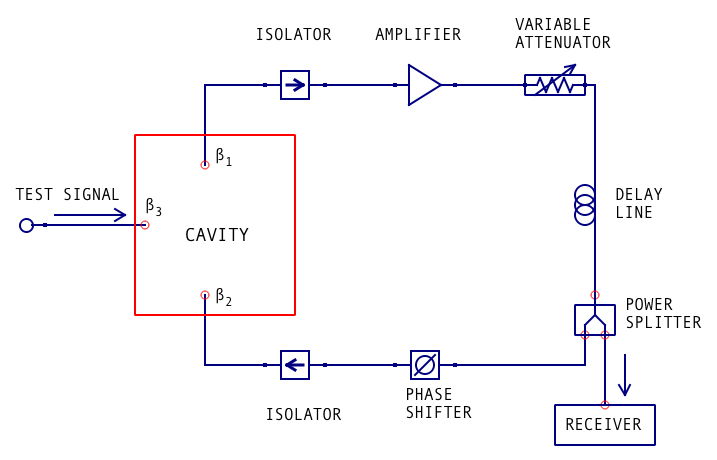
\includegraphics[width=\textwidth]{export_ouroboros}
%\column{0.5\textwidth}
%\begin{itemize}
%\item $t$: time around loop
%\item $\tau$: coherence time of cavity
%\item Intuition: signal feeds back coherently; when $t > \tau$, noise adds incoherently
%\end{itemize}
%\end{columns}
\end{frame}

\begin{frame}{People}
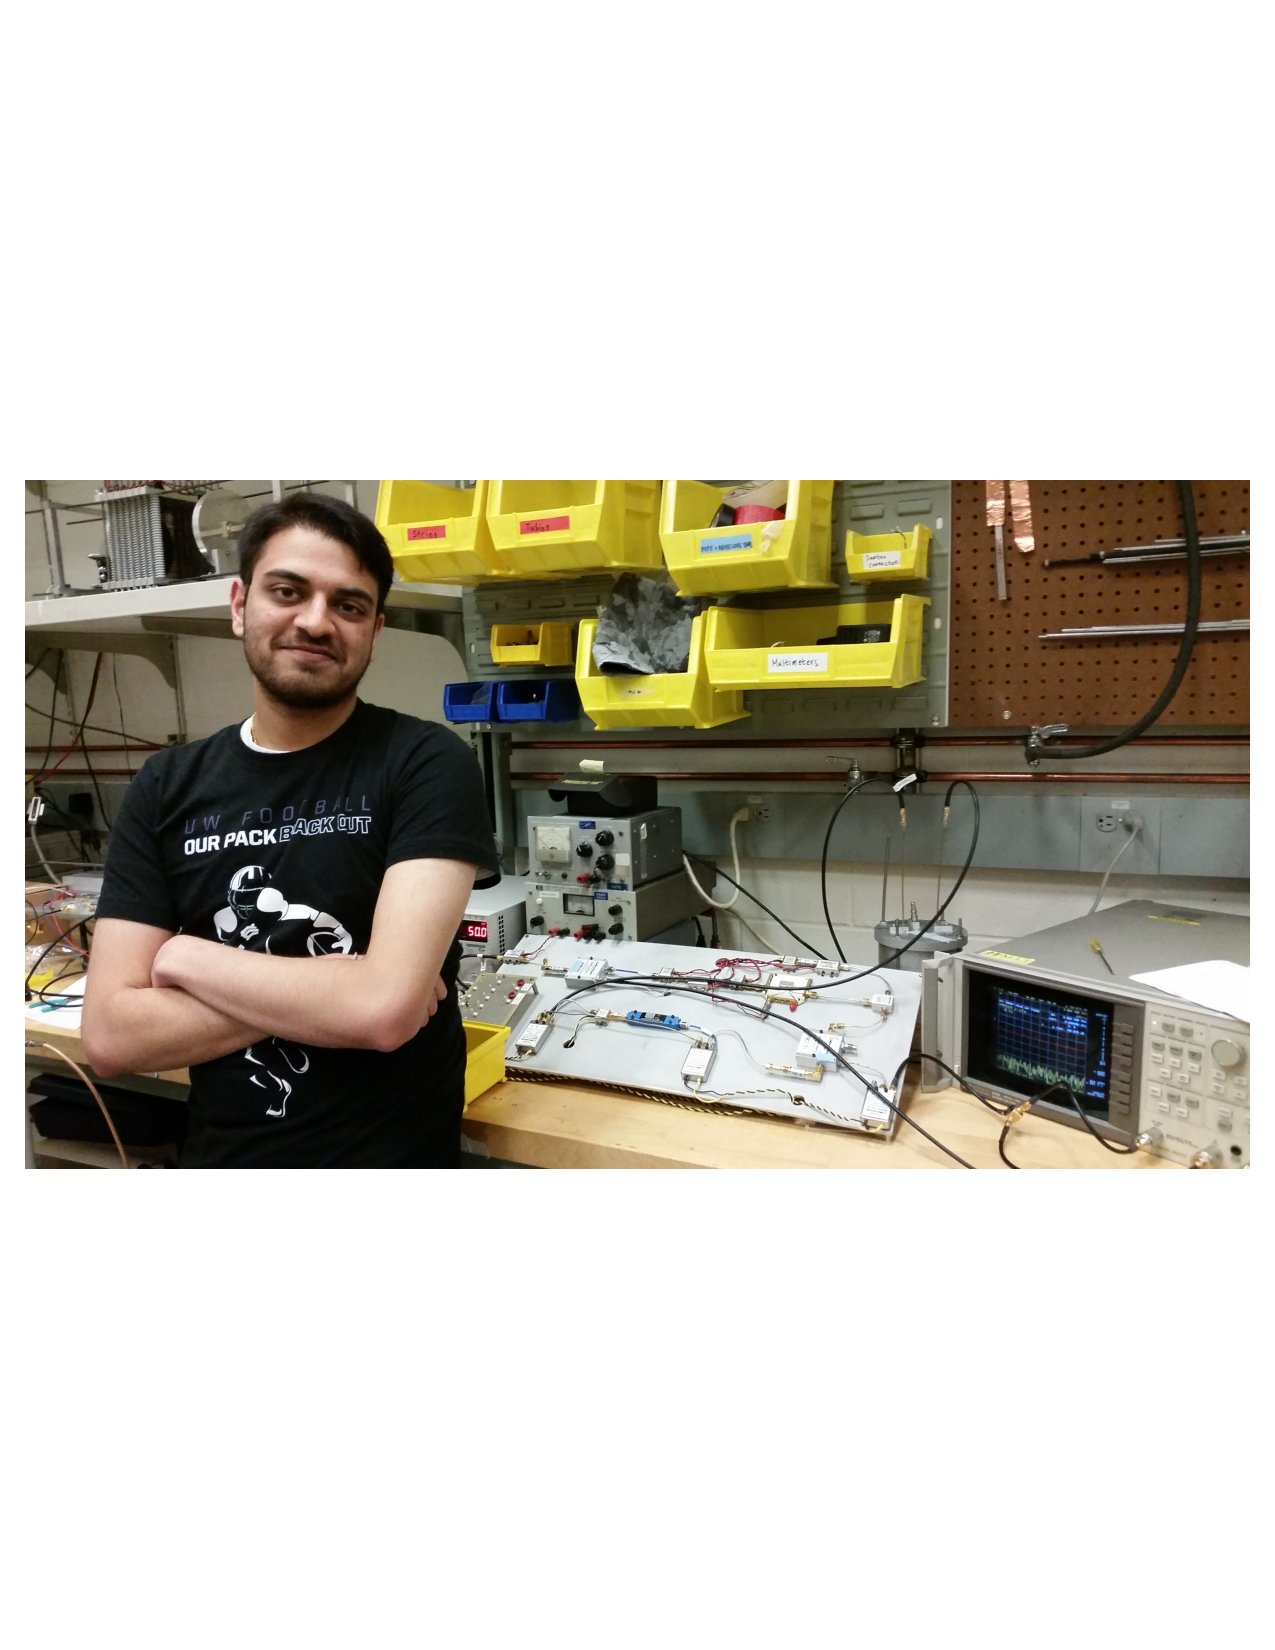
\includegraphics[width=\textwidth]{kunal_pic}
\end{frame}

\begin{frame}{Active Feedback Resonator}
{\tiny Ouroboros}
\begin{columns}
\column{0.5\textwidth}
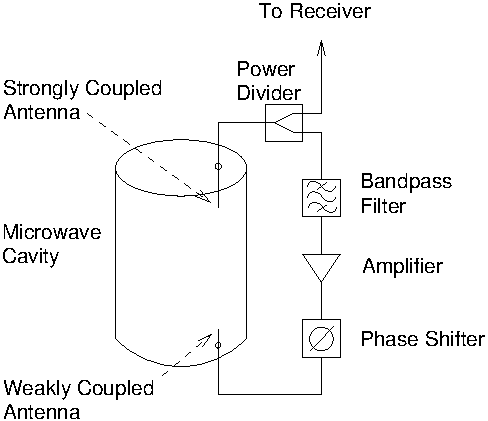
\includegraphics[width=\textwidth]{experiment_schematic-eps-converted-to}
\column{0.5\textwidth}
\begin{itemize}
\item $t$: time around loop
\item $\tau$: coherence time of cavity
\item Intuition: signal feeds back coherently; when $t > \tau$, noise adds incoherently
\end{itemize}
\end{columns}
\end{frame}

\begin{frame}{Equivalent Circuit}
\centering
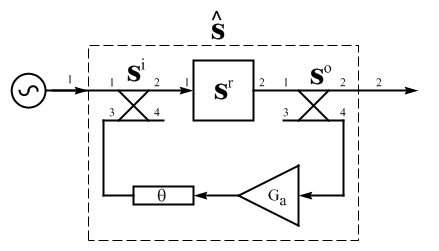
\includegraphics[width=.5\textwidth]{qmultiplier}

$G_l$ the loop gain\\
$Q_0$ the active quality factor\\
$T_a$ the amplifier noise temperature\\
%$T_{cav}$ the cavity noise temperature\\
\begin{columns}
\column{0.5\textwidth}
\centering
\begin{align*}
Q_0 = Q_L(1-\sqrt{G_l})^{-1} \\
|\hat{S}_{21}|^2 \propto (1- \sqrt{G_l})^{-2}
\end{align*}
\column{0.5\textwidth}
\centering
\begin{align*}
T_{noise} = \frac{T_{cav} + G_l T_a}{1 + G_l - 2\sqrt{G_l}e^{-t/\tau - i\theta}}
\end{align*}
\end{columns}
\end{frame}

\begin{frame}{Prototype}
\begin{columns}
\column{0.5\textwidth}
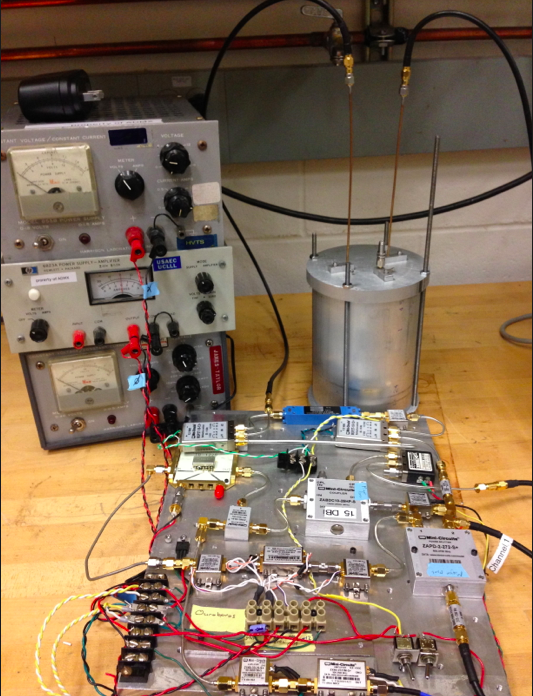
\includegraphics[width=\textwidth]{active_resonator_setup_photo}
\column{0.5\textwidth}
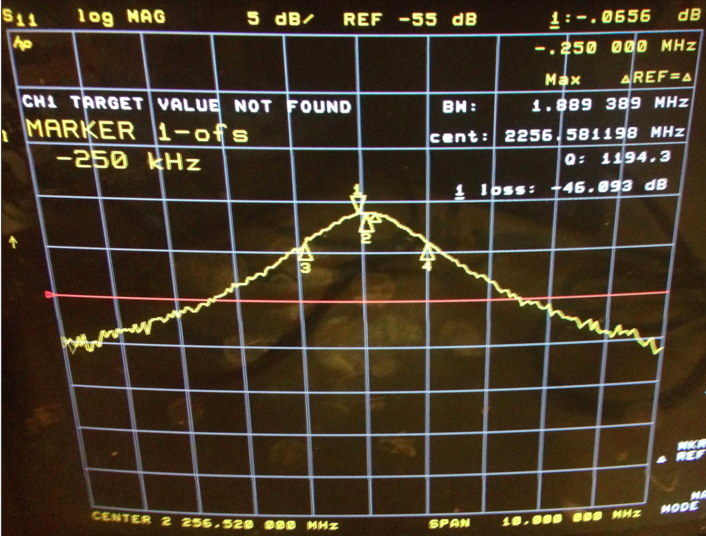
\includegraphics[width=\textwidth]{s21_no_delay}

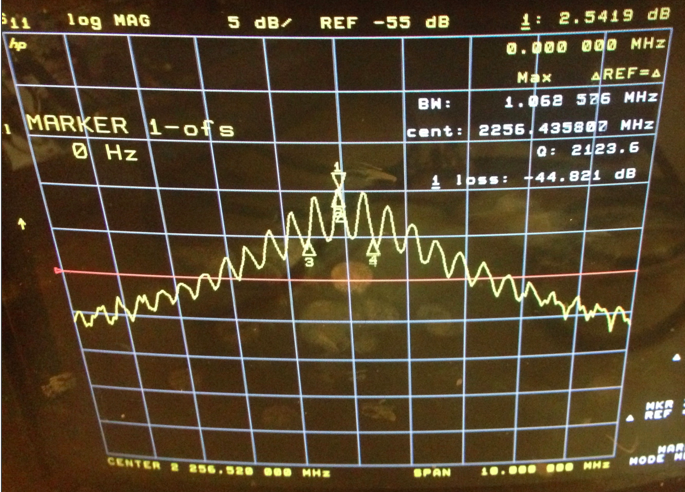
\includegraphics[width=\textwidth]{s21_delay}
\end{columns}

\end{frame}

\begin{frame}{Results}
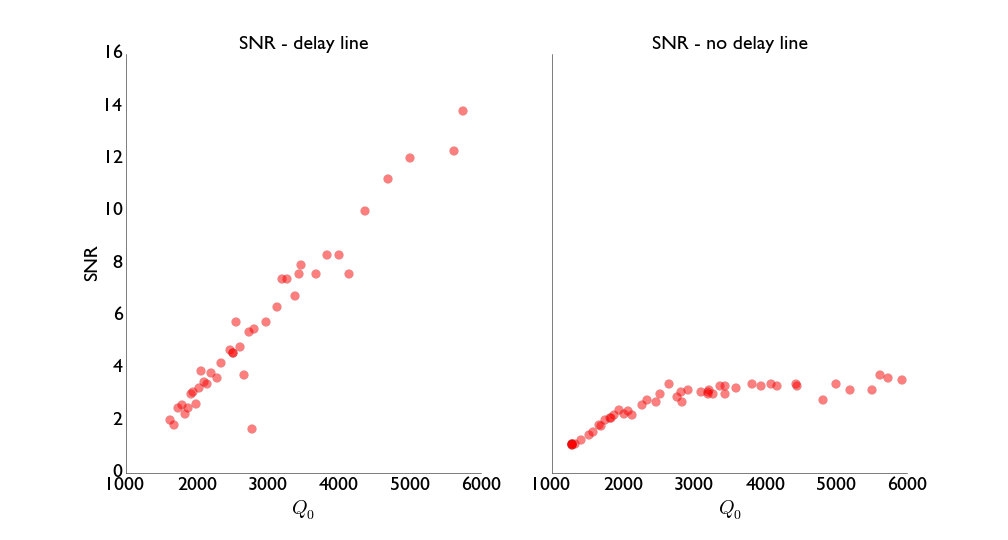
\includegraphics[width=\textwidth]{summary_plots}
\end{frame}

\end{document}